\documentclass[border=10pt,12pt]{standalone}

\usepackage{pgf}
\usepackage{tikz}
\usetikzlibrary{arrows,shapes,snakes}
\usetikzlibrary{shapes.multipart}

\begin{document}

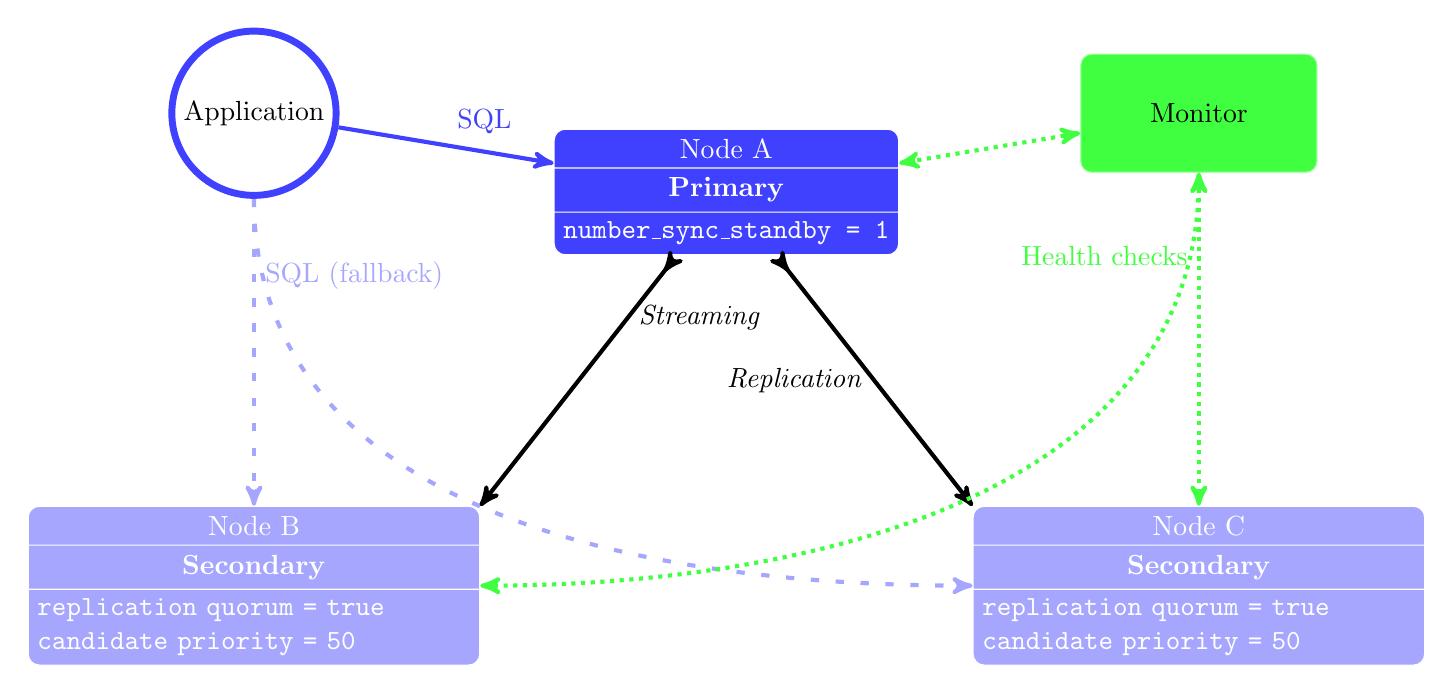
\begin{tikzpicture}[>=stealth',auto,rounded corners]

  \tikzstyle{app}=[circle,thick,draw=blue!75,fill=white,line width=0.25em]
  \tikzstyle{primary}=[rectangle split,rectangle split parts=3,
    text=white,draw=white,fill=blue!75,
    minimum height=3cm,minimum width=4cm]
  \tikzstyle{standby}=[rectangle split,rectangle split parts=3,
    draw=white,fill=blue!35,text=white,
    minimum height=1.75cm,minimum width=3cm]
  \tikzstyle{monitor}=[draw=green!35,fill=green!75,
    minimum height=1.5cm,minimum width=3cm]

  %% \draw [help lines] (-10,0) grid (10,20);

  \node  (a)   at (0,17)   [primary]
         {Node A
           \nodepart{second}
           \textbf{Primary}
           \nodepart{third}
           \texttt{number\_sync\_standby = 1}
         };

  \node  (b)   at (-6,12)  [standby,text width=5.5cm,align=center]
         {Node B
           \nodepart{second}
           \textbf{Secondary}
           \nodepart[align=left]{third}
           \texttt{replication quorum = true} \\
           \texttt{candidate priority = 50}
         };

  \node  (c)   at (6,12)   [standby,text width=5.5cm,align=center]
         {Node C
           \nodepart{second}
           \textbf{Secondary}
           \nodepart[align=left]{third}
           \texttt{replication quorum = true} \\
           \texttt{candidate priority = 50}
         };

  \node  (app) at (-6,18)  [app]        {Application};
  \node  (m)   at (6,18)   [monitor]    {Monitor};

  \tikzstyle{sql}=[->,color=blue!75,line width=0.15em]
  \tikzstyle{sqlf}=[->,color=blue!35,line width=0.15em,loosely dashed]
  \tikzstyle{sr}=[>->,line width=0.15em]
  \tikzstyle{hc}=[<->,color=green!75,line width=0.15em,dotted]

  \path (app) edge [sql]  node {SQL}                              (a)
              edge [sqlf] node[right,near start] {SQL (fallback)} (b)
              edge [sqlf,out=-90,in=180]                          (c)

        (a)   edge [sr]  node[right,near start]  {\textit{Streaming}}   (b.north east)
              edge [sr] node[left] {\textit{Replication}} (c.north west)

        (m)   edge [hc]                                               (a)
              edge [hc,out=-90,in=0]                                  (b)
              edge [hc] node[left,near start] {Health checks}         (c);
\end{tikzpicture}

\end{document}
